\chapter{CPLEX implementation and performance}

\section{CPLEX}
IBM ILOG CPLEX Optimizer is a solver licensed software, part of the IBM ILOG Optimizer Studio, with high level of efficiency and robustness \cite{IBMILOGCPLEX}. It can resolve a wide variety of problems:
\begin{itemize}
	\item Linear Programming (LP)
	\item Network Flow,
	\item Quadratic Programming (QP),
	\item Quadratically Constrained Programming (QCP),
	\item Mixed Integer Programming (MIP).
\end{itemize}
The interest, for the course purposes, is the LP optimization used to solve the TSP problem. The library written in C language, allow to define and resolve LP models with different heuristics and exact algorithm. The challenge is to implement with a state of the art LP solver the models specified in the chapter \ref{chapter:TSPdescription}, comparing time performance. 

\subsection{Callback}
\subsubsection{Lazy callback}
\subsubsection{Generic callback}



\section{Subtour Elimination}\label{sec:subtour}
The subtour elimination model described above enhance an exponential number of constraint ($ O(2^n) $), therefore it is not practicable to insert all the constraint in the model definition, instead is preferable to resolve the continuous relaxation without subtour elimination and than check if the solution verify the constraints, otherwise add the more violated constraints to the model. Four different version of subtour elimination model has been created:
\begin{enumerate}
	\item \textit{subtour\_iter\_opt}: the iteration apply the optimization step (\textit{CPX\_mipopt()}) and externally check the subtour constraints and eventually add the violated to the model. When no constraint is violated the best solution is found.
	\item \textit{subtour\_heur\_iter\_opt}: is equal to the previous one, but for the first iteration the subtour check is done immediately after the first available solution is found.
	\item \textit{subtour\_callback\_lazy}: While in the first two method the check is done outside CPLEX, here are used the \textit{CPXaddlazyconstraints()} which allow to check the constraints each time an incumbent should be update and to add the violated ones.
	\item \textit{subtour\_callback\_general}: The \textit{CPXcallbacksetfunc()} allow to set up a callback specifying the context in which to call that function. In this method is used to apply the lazy constraint with \textit{CPXcutcallbackadd()} in the \textit{CPX\_CALLBACKCONTEXT\_CANDIDATE} context.
\end{enumerate} 

\begin{figure}[h]
	\begin{subfigure}{.5\textwidth}
		\centering
		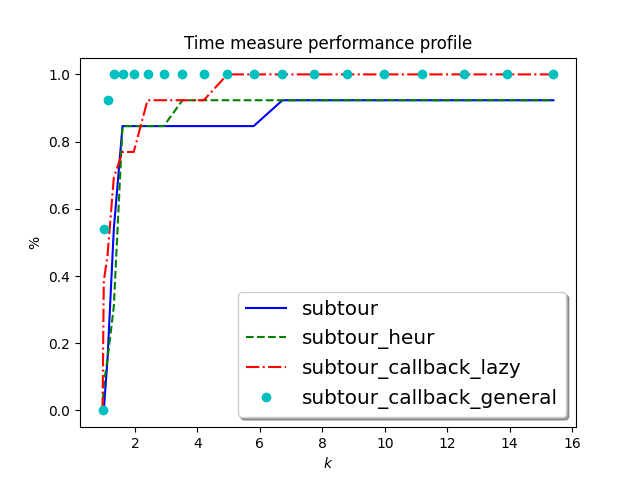
\includegraphics[width=\columnwidth]{../res/Lsubtours_average_time.png}
		\caption{Performance profile of the Data Average set}
		\label{fig:res_subtour_av}
	\end{subfigure}
	\begin{subfigure}{.5\textwidth}
	\centering
	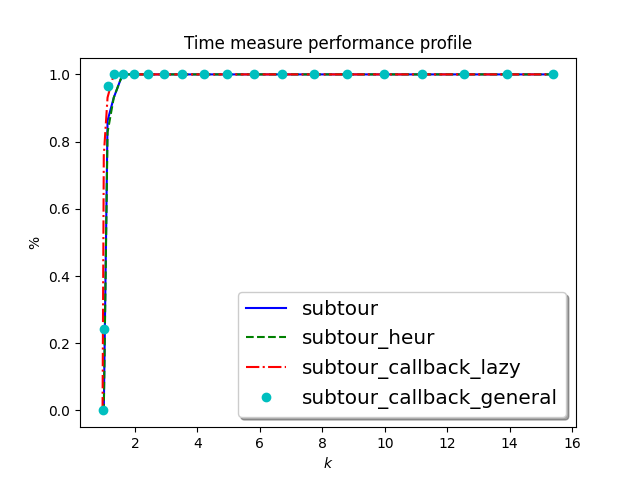
\includegraphics[width=\columnwidth]{../res/Lsubtours_light_time.png}
	\caption{Performance profile of the Data Light set}
	\label{fig:res_subtour_li}
	\end{subfigure}
\end{figure}

The performance profile in figure \ref{fig:res_subtour_av} is obtained by executing each subtour method in each Data Average instance for 5 different random seed generator. It show that in the $ 80\%  $  of the instances the \textit{subtour\_callback\_general} perform better than the other 3 alternatives.

qualche ulteriore dettaglio implementativo

confronto tra user callback e generic callback 

performance profile


\section{Miller Tucker Zemlin}

considerazioni sul numero di vincoli e sul problema asimmetrico

dettagli implementativi


\section{Flow Chart}

considerazioni sul numero di vincoli e sul problema asimmetrico

dettagli implementativi

performance profile con MTZ
